\documentclass{article}


\usepackage{arxiv}

\usepackage[utf8]{inputenc} % allow utf-8 input
\usepackage[T1]{fontenc}    % use 8-bit T1 fonts
\usepackage{hyperref}       % hyperlinks
\usepackage{url}            % simple URL typesetting
\usepackage{booktabs}       % professional-quality tables
\usepackage{amsfonts}       % blackboard math symbols
\usepackage{nicefrac}       % compact symbols for 1/2, etc.
\usepackage{microtype}      % microtypography
\usepackage{lipsum}
\usepackage{fancyhdr}       % header
\usepackage{graphicx}       % graphics
\graphicspath{{media/}}     % organize your images and other figures under media/ folder

%Header
\pagestyle{fancy}
\thispagestyle{empty}
\rhead{ \textit{ }} 

% Update your Headers here
\fancyhead[LO]{Running Title for Header}
% \fancyhead[RE]{Firstauthor and Secondauthor} % Firstauthor et al. if more than 2 - must use \documentclass[twoside]{article}



  
%% Title
\title{Generating Synthetic Data via Intent-Preserving and Intent-Corrupting Augmentations for Training Dialogue Embeddings.
%%%% Cite as
%%%% Update your official citation here when published 
\thanks{\textit{\underline{Citation}}: 
\textbf{Authors. Title. Pages.... DOI:000000/11111.}} 
}

\author{
  Author1, Author2 \\
  Affiliation \\
  Univ \\
  City\\
  \texttt{\{Author1, Author2\}email@email} \\
  %% examples of more authors
   \And
  Author3 \\
  Affiliation \\
  Univ \\
  City\\
  \texttt{email@email} \\
  %% \AND
  %% Coauthor \\
  %% Affiliation \\
  %% Address \\
  %% \texttt{email} \\
  %% \And
  %% Coauthor \\
  %% Affiliation \\
  %% Address \\
  %% \texttt{email} \\
  %% \And
  %% Coauthor \\
  %% Affiliation \\
  %% Address \\
  %% \texttt{email} \\
}


\begin{document}
\maketitle


\begin{abstract}
Text embeddings from pre-trained language models have been proven to be extraordinarily useful for various sentence-level tasks, such as pair classification, similarity estimation, and retrieval. Corresponding models are usually trained on large amounts of clean and diverse data using contrastive loss. Unfortunately, there are no such datasets for the domain of dialogue data. In this work, we describe the process of mining a synthetic dataset of dialogues for contrastive learning with hard negatives. We investigate various augmentation strategies for constructing dialogues with preserved or corrupted intents (positive and negative samples, respectively). To demonstrate the stated cleanliness and diversity, we train a dialogue encoder model and analyze its properties.
\end{abstract}


% keywords can be removed
\keywords{text embedding \and dialogue \and synthetic data \and text augmentation}


\section{Introduction}
Obtaining embeddings is one of the key themes in machine learning as a whole, and a popular task in recent years. Vector representation of an object is a convenient mathematical entity. If an embedding accurately and comprehensively encodes the semantics of the original data, it opens up the possibility of using it in a wide range of tasks.

In the field of natural language processing, classical methods for text vectorization such as bag of words \cite{bow} and tf-idf \cite{SprckJones2021ASI} have long been invented. Thanks to deep learning, we have witnessed remarkable word vectorizations for their time, such as word2vec \cite{mikolov2013efficient} and GloVe \cite{pennington-etal-2014-glove}, which convey the semantic similarity between words; CoVe \cite{mccann2018learned} and ELMo \cite{peters-etal-2018-deep}, which provide information about the surrounding context. Recently, powerful encoder models have emerged that produce general-purpose text embeddings \cite{xiao2023cpack, wang2022text, li2023general}. They incorporate so much semantic information about texts that it can be applied to tasks such as classification, clustering, ranking, semantic textual similarity, and more. The success of these models is largely attributed to the use of contrastive learning on massive datasets. 

However, the more specific the data structure, the more challenging it is to mine a large dataset. As of today, there are no encoding methods for dialogue data. In other words, there is no way to obtain a dense vector representation that conveys universal information about a dialogue. There are language models that adapt successfully to the hierarchical and temporal nature of dialogue \cite{zhang-etal-2023-dialog, li2022future}, but they only address tasks at the token and utterance levels, not at the dialogue level. This is due to the lack of datasets that pose challenges at the dialogue level.

Data is almost always scarce when it comes to building dialogue models. To date, numerous methods for generating synthetic dialogues have been devised \cite{kim2021neuralwoz, mohapatra2021simulated, wan-etal-2022-unified, zheng2023augesc}, but they do not generate dialogues in pairs \cite{schick2021generating}, as is conceptually important for contrastive embedding learning. The simplest way to expand a training dataset is through augmentation \cite{soudani2023data}. However, we find them insufficient, as they do not significantly alter the structure of the dialogue. In this work, we will describe a method for constructing a synthetic dataset of dialogue pairs using various augmentations that preserve or alter the set of intents in the dialogue. These augmentations significantly affect its structure.


\section{Approach}

\subsection{Augmentations}

\textbf{Token Insertion.} One of the simple yet effective ways to augment text is to lengthen it by inserting additional tokens. For this purpose, we added a special token `<mask>` to random places in the dialogues and used transformer models trained on the MLM task to fill these masks. Insertion was rejected if the token proposed by the model was only a fragment of a word (BPE, Wordpiece) or if the prediction probability was below a manually set threshold. To take the dialogue context into account during token insertion, multiple consecutive responses or the entire dialogue were fed into the MLM model at once.

\textbf{Token Replacement.} This method is identical to the previous one, except that instead of adding the `<mask>` token between tokens in the original dialogue, some tokens in the original dialogue are replaced.

\textbf{Back Translation.} Translation from the original language to another language and then back to the original language. MT models were used for this purpose.

\textbf{Shuffling Responses.} Previous augmentations modify the dialogue within individual phrases since they are methods applicable to arbitrary text data. It seems essential to learn how to change the order of responses in a dialogue to create a valid example of meaningful dialogue. For this purpose, we propose using models that measure the similarity between responses within a dialogue \ref{fig:pairwise}. Using these distances, it is possible to cluster responses within each dialogue. Experiments showed that these clusters represent significant individual stages of the dialogue that can be shuffled with each other.

\begin{figure}[!htb]
    \centering
    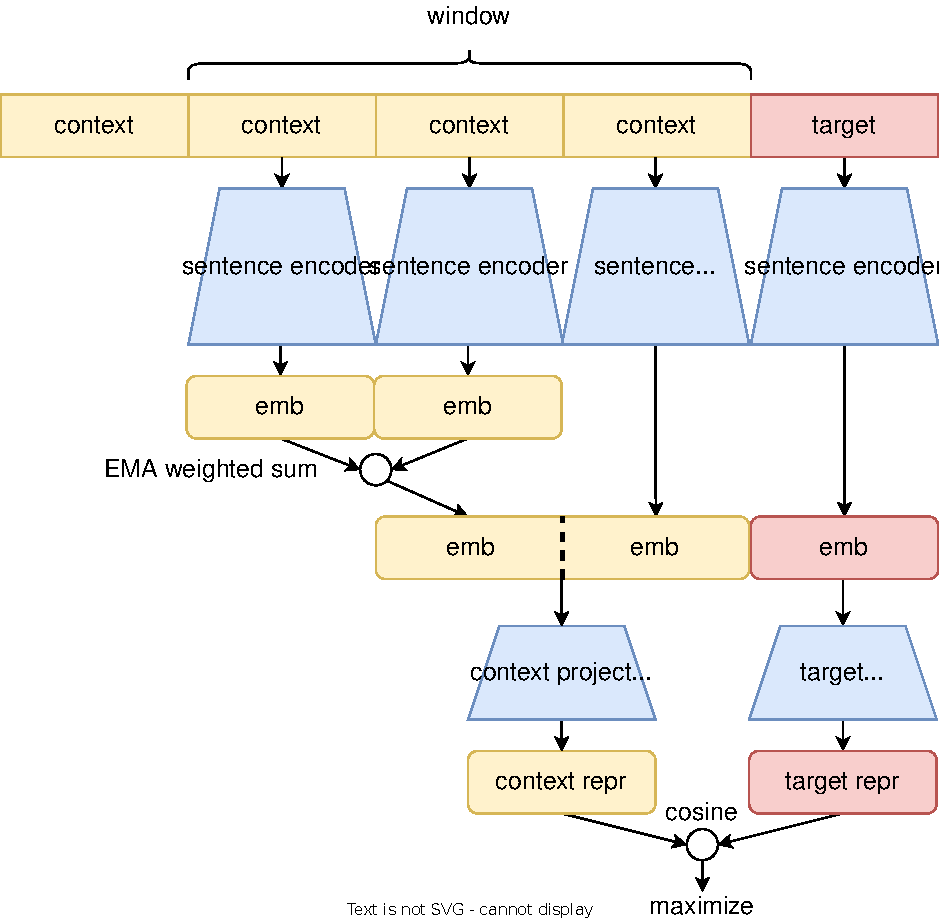
\includegraphics[width=0.7\linewidth]{figures/dialogue-shufflers-pairwise.drawio.pdf}
    \caption{Model for measuring the distance between responses in a dialogue.}
    \label{fig:pairwise}
\end{figure}

\textbf{Shortening the Dialogue.} Individual clusters of responses within the dialogue can be discarded, resulting in a dialogue with fewer responses.

\textbf{Lengthening the Dialogue.} A model was trained to arrange responses in a dialogue based on a given list of responses. This transformer takes the text embeddings of each response as input without specifying information about the position of the response in the original dialogue. It outputs ranks or probabilities that can be used to "sort" the responses. If some external responses are added to the original dialogue, this model generates a new, longer dialogue.

\begin{figure}[!htb]
    \centering
    \includegraphics[width=0.7\linewidth]{figures/dialogue-shufflers-listwise-lm-1.drawio.pdf}
    \caption{Model for extending the dialogue through sorting.}
    \label{fig:listwise}
\end{figure}

\textbf{Preserving and Altering Intent.} The augmentations mentioned above can be configured to either preserve or alter intent. As augmentations that preserve intent, we used all operations except token replacement, which was used to select hard negative examples.

\subsection{Dialogue Encoder}

\textbf{BERT.} As a baseline method for vectorization, we use BERT without any modifications. We input the dialogue as \texttt{[CLS] ut1 [SEP] ut2 [SEP] ut3 [SEP]}, and the output is the averaged vectors of the hidden state of the `SEP` tokens.

\textbf{HSSA and BiDeN.} For slightly advanced dialogue language models, we use HSSA and BiDeN.

For training dialogue encoders, we use contrastive learning with in-batch negative examples and hard negative examples:
$$
\mathcal{L}=-\log{\exp(\cos(x_i,y_i))\over\sum_{j=1}^B\exp(\cos(x_i,y_j))},
$$


\section*{Acknowledgments}
This was was supported in part by......

%Bibliography
\bibliographystyle{unsrt}  
\bibliography{references}  


\end{document}
